
\chapter{实验结果}
\label{cha:experiment}

在本章中,我们完整地展示了 F2000 模式分量的代码生成、编译、运行、数据分析等步骤。

\section{配置文件}

\usetikzlibrary{trees}
\tikzstyle{every node}=[draw=black,thick,anchor=west]
\tikzstyle{selected}=[draw=red,fill=red!30]
\tikzstyle{optional}=[dashed,fill=gray!50]
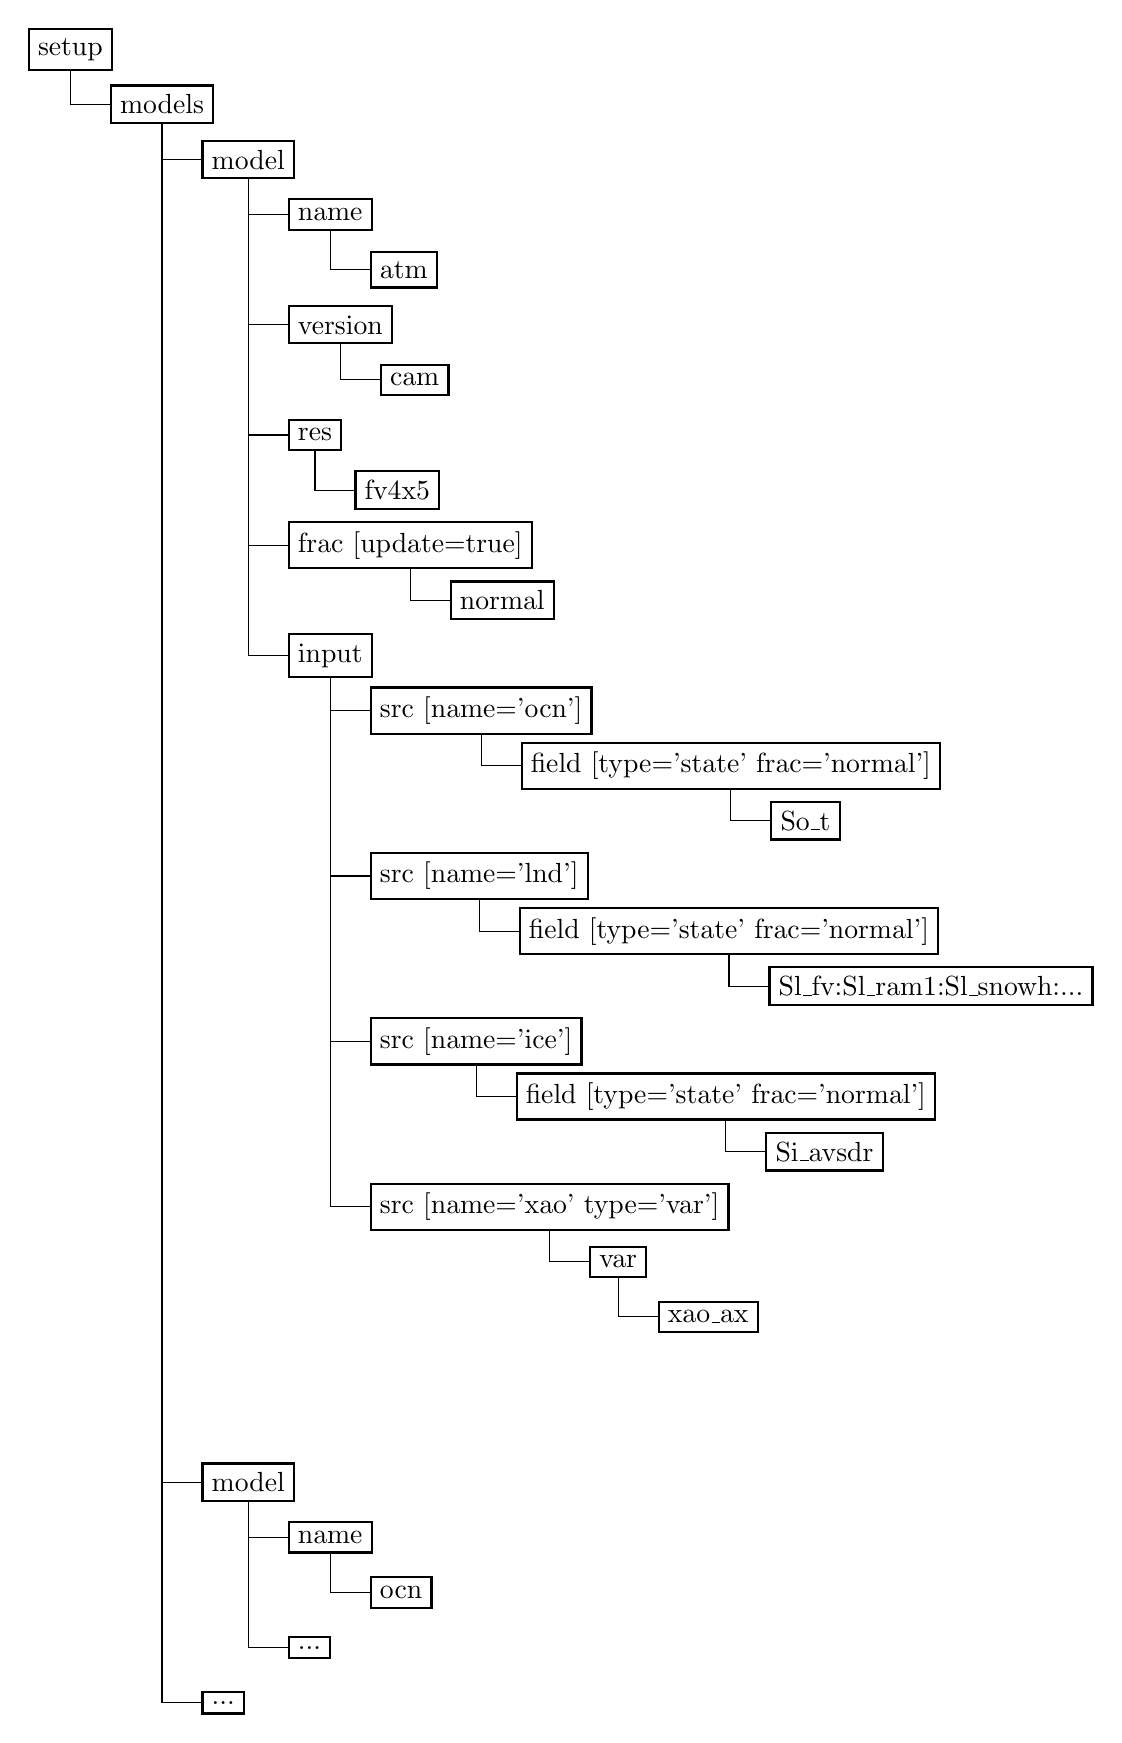
\begin{tikzpicture}[%
  grow via three points={one child at (0.5,-0.7) and
  two children at (0.5,-0.7) and (0.5,-1.4)},
  edge from parent path={(\tikzparentnode.south) |- (\tikzchildnode.west)}]
  \node {setup}
    child { node {models} 
      child { node {model}
        child { node {name}
          child { node {atm} }
        }
        child [missing] {}
        child { node {version}
          child { node {cam} }
        }
        child [missing] {}    		
        child { node {res}
          child { node {fv4x5} }
        }
        child [missing] {}
        child { node {frac [update=true]}
          child { node {normal} }
        }
        child [missing] {}
        child { node {input}
          child { node {src [name='ocn']} 
          	child { node {field [type='state' frac='normal']}
          	  child {node {So\_t}}
          	}
          	child [missing] {}          	
          }
          child [missing] {}
          child [missing] {}
          child { node {src [name='lnd']} 
          	child { node {field [type='state' frac='normal']}
          	  child {node {Sl\_fv:Sl\_ram1:Sl\_snowh:...}}
          	}
          	child [missing] {}          	
          }
          child [missing] {}
          child [missing] {}
          child { node {src [name='ice']} 
          	child { node {field [type='state' frac='normal']}
          	  child {node {Si\_avsdr}}
          	}
          	child [missing] {}          	
          }
          child [missing] {}
          child [missing] {}          
          child { node {src [name='xao' type='var']} 
          	child { node {var}
          	  child {node {xao\_ax}}
          	}
          	child [missing] {}      	
          }
          child [missing] {}
          child [missing] {}        }
        child [missing] {}
      }
      child [missing] {}
      child [missing] {}
      child [missing] {}
      child [missing] {}
      child [missing] {}
      child [missing] {}
      child [missing] {}
      child [missing] {}
      child [missing] {}
      child [missing] {}
      child [missing] {}
      child [missing] {}
      child [missing] {}
      child [missing] {}
      child [missing] {}
      child [missing] {}
      child [missing] {}
      child [missing] {}
      child [missing] {}
      child [missing] {}
      child [missing] {}
      child [missing] {}
      child [missing] {}
      child { node {model}
        child { node {name}
          child { node {ocn} }
        }
        child [missing] {}
        child { node {...} }
      }
      child [missing] {}
      child [missing] {}
      child [missing] {}
      child { node {...} } 
    };
\end{tikzpicture}
